\section*{Contributions}
\addcontentsline{toc}{section}{\protect\numberline{}Main results}

\begin{figure}[h]
  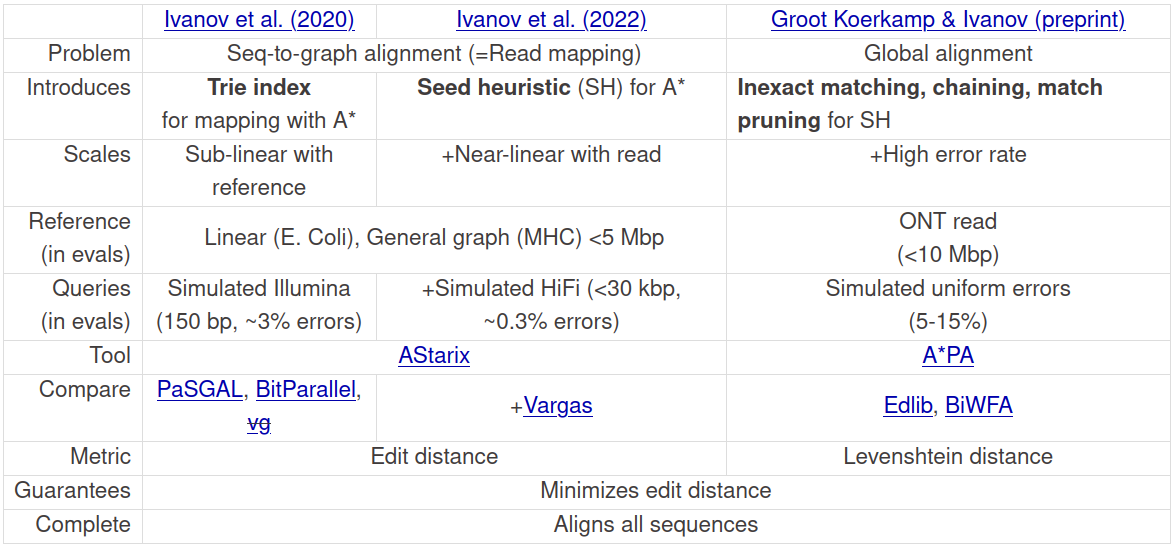
\includegraphics[width=1.0\linewidth]{media/ownpubs-table.png}
  \caption{Overview of the contributions by publication. \cref{ch:trie}
  corresponds to \citep{ivanov2020astarix}, \cref{ch:seed} to
  \citep{ivanov2022fast}, \cref{ch:global} to \citep{koerkamp2022exact}}
  \label{tab:ownpubs}
\end{figure}

% Optimality, heuristic speed
In this thesis we introduce a novel principled approach for provably optimal and
heuristically fast sequence alignment. The underlying idea of this thesis is to
speed up the search of an optimal alignment using information from the whole
sequences, and not only from the aligned parts as existing algorithms do. We
apply our approach to sequence-to-graph semi-global alignment (for read mapping)
and global alignment. The question that we target is how general can the input
sequences be while we could still efficiently compute provably-optimal
alignments. To this end, we introduce novel algorithmic and data structure
techniques, prove their correctness, and implement them as free and open source
tools. Our evaluations demonstrate that remarkable performance scaling up to
huge references, very long queries/sequences and high error rates. In absolute
terms, we demontrate orders of magnitude of speedup compared to existing optimal
algorithm on synthetic and real data.

\subsection*{Methods}

\paragraph{\A for sequence alignment}
We consider the sequence alignment problem in its principled and powerful graph
formulation: an alignment minimizing edit distance is equivalent to a shortest
path in an \emph{alignment graph}. It allows to choose any shortest path
algorithm, and, assuming non-negative edit costs, we select the \A algorithm for
its ability to use any available information to quickly direct the search and
yet, to guarantee optimality. In order to efficiently apply \A to semi-global
and global alignment, we complement the reference with a trie index, design a
powerful \emph{seed heuristic}, and implement a number of algorithmic
optimizations. We formally prove the optimality of all algorithms, data
structures, and optimizations.

\paragraph{Implicit constructiong of the alignment graph}
The alignment graph is defined as a Cartesian product of the reference and the
query. The structure of the alignment graph is thus regular, and we do not have
to build it explicitly but to only constuct it locally at the node we are
exploring. This optimization is crucial for the overall performance of \A which
spends time only at explored nodes before terminating at the target.

\paragraph{Sequence-to-graph alignment}
Unlike most dynamic programming solutions, we are not bound to acyclic graphs
due to using the general \A shortest path algorithm. Thus, our reference is not
limited to being a linear sequence but can as well be any genome graph. All
semi-global alignment algorithms in this thesis are applicable to general graphs
(possibly including cycles).

\paragraph{Scaling with reference size using a trie index}
In~\cref{ch:trie} we suggest how to exploit that many query sequences are
semi-globally aligned to the same reference. As a preprocessing step, we
complement the reference with a trie index (similar to a suffix tree) so that
any kmer from the reference appears as a path from the trie root to a trie leaf,
and then links to the reference. This way, any substring in the trie is a spell
of a path from the trie root. With an accurate heuristic function (i.e.
estimating the remaining edit distance well), this trie complement allows to
ignore most of the reference.

\paragraph{Scaling with query length using seed heuristic}
In~\cref{ch:seed} we introduce a powerful \emph{seed heuristic} for \A. It
estimates the remaining edit distance based on information from the whole
reference and query, we prove its admissibility, and present an algorithm for
its efficient computation.

In order to quickly compute the seed heuristic for any explored state by \A, we
first precompute.

We borrow the existing concept of seeds but apply it in a novel way: instead of
finding alignments around seed matches, we use the lack of matches to penalize
alignments by desigining the \emph{seed heuristic} that drive the \A search.

In addition to the trie index to scale with reference size, 

To ensure that our algorithms are practical, we introduce a number of
algorithmic optimizations which increase performance and decrease memory
footprint.
%

\paragraph{Scaling with error rate using chaining, inexact matching and gap costs}
In~\cref{ch:global} we. The specifics with semi-global alignment requires a
trie-like index which is well-used in the fields, and known since
\citeyear{thue1912gegenseitige}~\cite{thue1912gegenseitige} and used in
informatics since~\citeyear{de1959file}~\cite{de1959file}.

\paragraph{Optimizations} Greedy matching

\paragraph{Implementations}
\astarix and \astarpa, minSH

Minimalistic: 

def build_seedh(A, B, k):
    seeds = [ A[i:i+k] for i in range(0, len(A)-k+1, k) ]           # O(n)   
    kmers = { B[j:j+k] for j in range(len(B)-k+1) }                 # O(nk), O(n) with rolling hash (Rabin-Karp)
    is_seed_missing = [ s not in kmers for s in seeds ] + [False]*2 # O(n)
    suffix_sum = np.cumsum(is_seed_missing[::-1])[::-1]             # O(n)
    return lambda ij, k=k: suffix_sum[ ceildiv(ij[0], k) ]          # O(1)

h_seed = build_seed_heuristic(A, B, k=log(len(A)))
astar(A, B, h_seed)
\subsection*{Results}

We empirically demonstrate the superior scaling and performance to other optimal
alignment algorithms.

\paragraph{Scaling with reference size using a trie index}
\paragraph{Scaling with query length using a seed heuristic}
\paragraph{Scaling with error rate using inexact matching and chaining}

% background
Traditionally, the runtime and memory have been analysed for the worst case
asymptotic behavior of the algorithm. Since the near quadratic worst case
asymptotics is likely to be tight for both global~\citep{backurs2015edit} and
semi-global alignment, we targeted related sequences (by limiting their
per-letter error rate), and estimated their empyric runtime and memory scaling.

% issue
The seed heuristic, which is in the core of our \A algorithm, is admissible
(optimistic) but not consistent (monotone). As a consequence, any of the
quadratic number of state can be expanded multiple times, which could
theoretically lead to over-quadratic scaling. In practice, repeated expansions
happen but the empyrical scaling is preserved near-linear as long as the number
of seed matches is near-linear and the seed heuristic is capable of compensating
for the errors.

% empyrical
Our empyrical analysis of scaling is done by repeatedly running the same
algorithm on increasingly more complex input data (\AG longer sequences, higher
error rate). This approach is useful to get a sense of the scaling of the
algorithm and its implementation but it is not asymptotical, includes noise (of
measurements and best-fit estimations), is not trivially applicable to more than
1 dimensions.

% theory
An alternative theoretical analysis would consider the average case (expected)
scaling of our algorithms under a data model. An imaginable result would look
like a connection between the sequence lengths, error rate, and the algorithm
steps (mostly dependant on the number of seed matches and the number of expanded
states). To construct such a connection, a heuristic function will have to be
chosen among a class of seed heuristics (\AG with certain seed length, allowed
number of errors in seed matches, etc.).

% regimes
Our algorithms seem to follow any of the scaling regimes, based on the
capability of the seed heuristic to compensate for all the errors.

% speculations
Based on the empitical evaluations and the intuition behind the algorithms, we
speculate that the sequence length until which our algorithms can scale
near-linearly, can be exponentially increased by lowering the error rate. For
the semi-global alignment, any unit of alignment cost that is not compensated by
the potential of the seed heuristic, leads to a deeper exploration of the trie,
which is grows exponentially until it saturate to quadratic.

\paragraph{Scaling with reference size}
In~\cref{ch:trie} we present the tool \astarix which applies the \A algorithm to
find optimal alignments, based on a domain-specific heuristic and enhanced by
multiple algorithmic optimizations. Importantly, our approach allows for both
cyclic and acyclic graphs including variation and de Bruijn graphs. We
demonstrate that using a trie index we can achieve sublinear scaling of aligning
runtime with reference size, and that \A can scale exponentially better than
\dijkstra with increasing (but small) number of errors in the reads. Moreover,
for short reads, both \astarix and \dijkstra scale better and outperform current
state-of-the-art optimal aligners with increasing genome graph size.
Nevertheless, scaling optimal alignment of long reads on big graphs remained an
open problem.

\paragraph{Scaling with query length}
In~\cref{ch:seed} we upgrade \astarix with a novel \sh which guides the \A
search by preferring crumbs on nodes that lead towards optimal alignments even
for long reads. This approach enables the scaling of semi-global alignment with
read length.

\paragraph{Scaling with error rate}
In~\cref{ch:global} we resolve the third major bottleneck -- handling high error
rates. We presented an algorithm with an implementation in \astarpa solving
pairwise alignment between two sequences. The algorithm is based on \A with a
\sh, inexact matching, match chaining, and match pruning, which we proved to
find an exact solution according to edit distance. For random sequences with up
to $15\%$ uniform errors, the runtime of \astarpa scales near-linearly to very
long sequences ($10^7\bp$) and outperforms other exact aligners. We demonstrate
that on real ONT reads from a human genome, \astarpa is faster than other
aligners on only a limited portion of the reads.
